\documentclass[12pt,a4paper]{report}

% =========================
% Packages
% =========================
\usepackage[utf8]{inputenc}
\usepackage[T1]{fontenc}
\usepackage[french]{babel}
\usepackage{lmodern}
\usepackage{geometry}
\usepackage{graphicx}
\usepackage{xcolor}
\usepackage{booktabs}
\usepackage{array}
\usepackage{tabularx}
\usepackage{longtable}
\usepackage{float}
\usepackage{caption}
\usepackage{subcaption}
\usepackage[hypertexnames=false]{hyperref}
\usepackage{bookmark}
\usepackage{listings}
\usepackage{fancyhdr}
\usepackage{setspace}
\usepackage{enumitem}
\usepackage{microtype}
\usepackage{wallpaper}

% Noms et styles des légendes
\addto\captionsfrench{%
  \renewcommand{\tablename}{Tableau}%
  \renewcommand{\listtablename}{Liste des tableaux}%
  \renewcommand{\figurename}{Figure}%
}
\renewcommand{\lstlistingname}{Code}
\captionsetup{font=small,labelfont=bf}

\geometry{margin=2.5cm}
\setlength{\headheight}{15pt}
\onehalfspacing
\graphicspath{{figures/}{tp1_ensias_cover_assets/}}

\definecolor{mainblue}{RGB}{27,76,130}
\definecolor{lightblue}{RGB}{235,244,255}
\definecolor{codebg}{RGB}{248,248,248}

\hypersetup{
    colorlinks=true,
    linkcolor=mainblue,
    citecolor=mainblue,
    urlcolor=mainblue,
    pdftitle={RetinaScan - Rapport de Projet de Fin d'Annee},
    pdfauthor={Bilal Erraki}
}

\pagestyle{fancy}
\fancyhf{}
\fancyhead[L]{RetinaScan}
\fancyhead[R]{Projet de Fin d'Année}
\fancyfoot[C]{\thepage}

\lstset{
    backgroundcolor=\color{codebg},
    basicstyle=\ttfamily\footnotesize,
    breaklines=true,
    frame=single,
    rulecolor=\color{gray},
    keywordstyle=\color{mainblue}\bfseries,
    commentstyle=\color{gray},
    stringstyle=\color{teal},
    showstringspaces=false,
    columns=fullflexible,
    keepspaces=true,
    tabsize=4
}

\newcommand{\projecttitle}{RetinaScan}
\newcommand{\projectsubtitle}{Classification de la rétinopathie diabétique à partir d'images du fond d'œil par Deep Learning}
\newcommand{\githublink}{https://github.com/bilal-erraki/RetinaScan}

\begin{document}

% =========================
% Page de garde
% =========================
\begin{titlepage}
\ThisLRCornerWallPaper{1}{tp1_ensias_cover_assets/background.png}
\centering


\includegraphics[width=0.28\textwidth]{tp1_ensias_cover_assets/ensias.png}\hfill

\includegraphics[width=0.28\textwidth]{tp1_ensias_cover_assets/um5logo.png}\par\vspace{1.1cm}

{\scshape\LARGE École Nationale Supérieure d'Informatique et\\ d'Analyse des Systèmes -- Rabat\par}
\vspace{1.35cm}

{\scshape\Large Rapport de Projet de Fin d'Année\par}
{\small\textit{Filière : Intelligence Artificielle}\par}
\vspace{0.9cm}

\rule{\linewidth}{0.2mm}\\[0.45cm]
{\huge\bfseries \projecttitle\par}
\vspace{0.25cm}
{\Large\bfseries Classification de la rétinopathie diabétique\\à partir d'images du fond d'œil par Deep Learning\par}
\rule{\linewidth}{0.2mm}\\[1.25cm]

\begin{minipage}{0.48\textwidth}
\begin{flushleft}\large
\textit{\textbf{\mbox{Réalisé par~:}}}\\
ERRAKI Bilal\\[0.35cm]
\textit{\textbf{\mbox{École~:}}}\\
ENSIAS
\end{flushleft}
\end{minipage}
\hfill
\begin{minipage}{0.42\textwidth}
\begin{flushright}\large
\textit{\textbf{\mbox{Encadrant~:}}}\\
Mr. LAZAAR Mohamed\\[0.35cm]
\textit{\textbf{\mbox{Technologies~:}}}\\
Python, TensorFlow/Keras, EfficientNetB3, FastAPI, Streamlit
\end{flushright}
\end{minipage}

\vspace{0.55cm}
{\large\textit{Code source :} \href{https://github.com/bilal-erraki/RetinaScan}{github.com/bilal-erraki/RetinaScan}\par}

\vfill
{\large 2025/2026\par}
\end{titlepage}

\pagenumbering{roman}

\chapter*{Remerciements}
Je tiens à exprimer ma reconnaissance à toutes les personnes qui ont contribué directement ou indirectement à la réalisation de ce projet. Je remercie particulièrement mon encadrant, Mr. LAZAAR Mohamed, pour son accompagnement et ses remarques durant l'avancement du travail. Je remercie également mes enseignants pour les connaissances acquises durant la formation, notamment dans les domaines de l'intelligence artificielle, du traitement d'images et du développement logiciel.

Ce projet m'a permis de relier plusieurs compétences étudiées pendant la formation : préparation des données, entraînement d'un modèle de Deep Learning, analyse critique des résultats et déploiement d'une solution simple sous forme d'API et d'interface web.

\chapter*{Résumé}
La rétinopathie diabétique est une complication du diabète qui touche les vaisseaux sanguins de la rétine. Sa détection précoce est essentielle afin de réduire le risque de perte de vision. Le projet \textbf{RetinaScan} a pour objectif de développer un système intelligent capable de classifier automatiquement des images du fond d'œil selon cinq niveaux de sévérité : No DR, Mild, Moderate, Severe et Proliferative DR.

La solution proposée repose sur l'apprentissage profond et la vision par ordinateur. Le modèle final implémenté utilise \textbf{EfficientNetB3} en transfert learning, avec une première phase où le backbone est gelé, puis une phase de fine-tuning. Le pipeline intègre le prétraitement des images, l'augmentation des données, la pondération des classes et la sauvegarde du meilleur checkpoint. Le modèle a ensuite été intégré dans une API d'inférence avec \textbf{FastAPI}, puis connecté à une interface utilisateur développée avec \textbf{Streamlit}. Les résultats finaux obtenus montrent une exactitude de validation de \textbf{78,58\%} et un \textbf{Quadratic Weighted Kappa de 0,8603}. Le modèle reconnaît très bien les classes No DR et Moderate, tandis que les classes Severe et Proliferative DR restent plus difficiles à cause du faible nombre d'exemples et de la similarité visuelle entre certains stades avancés.

\textbf{Mots-clés :} Deep Learning, Computer Vision, rétinopathie diabétique, EfficientNetB3, transfert learning, FastAPI, Streamlit.

\chapter*{Abstract}
Diabetic retinopathy is a diabetes-related complication affecting retinal blood vessels. Early detection is important to reduce the risk of vision loss. The \textbf{RetinaScan} project aims to build an intelligent system that automatically classifies fundus images into five severity levels: No DR, Mild, Moderate, Severe, and Proliferative DR.

The proposed solution is based on deep learning and computer vision. The final implemented model uses \textbf{EfficientNetB3} with transfer learning, a frozen-backbone training phase, fine-tuning, data augmentation, and class weighting to reduce the impact of dataset imbalance. The trained model was deployed through a \textbf{FastAPI} inference API and connected to a \textbf{Streamlit} user interface. The final validation accuracy obtained is \textbf{78.58\%}, with a \textbf{Quadratic Weighted Kappa of 0.8603}. The model performs very well on No DR and Moderate cases, while Severe and Proliferative DR remain more challenging due to data imbalance and visual similarity between advanced stages.

\textbf{Keywords:} Deep Learning, Computer Vision, diabetic retinopathy, EfficientNetB3, transfer learning, FastAPI, Streamlit.

\tableofcontents
\listoffigures
\listoftables
\newpage
\pagenumbering{arabic}

% =========================
\chapter{Introduction}

\section{Contexte général}
Le diabète est une maladie chronique pouvant provoquer plusieurs complications à long terme. Parmi celles-ci, la rétinopathie diabétique représente une atteinte de la rétine causée par l'endommagement progressif des vaisseaux sanguins. Lorsque cette maladie n'est pas détectée et suivie correctement, elle peut entraîner une baisse importante de la vision, voire la cécité.

Le diagnostic de la rétinopathie diabétique repose généralement sur l'analyse d'images du fond d'œil par des spécialistes. Cependant, l'analyse manuelle peut être longue, coûteuse et dépendante de la disponibilité des ophtalmologues. Dans ce contexte, l'intelligence artificielle et la vision par ordinateur peuvent constituer une aide utile pour automatiser une partie du processus d'analyse.

\section{Problématique}
La problématique principale de ce projet est la suivante :

\begin{quote}
\textit{Comment développer un système de Deep Learning capable de classifier automatiquement des images du fond d'œil selon le stade de rétinopathie diabétique, tout en tenant compte de la complexité des images médicales et du déséquilibre des classes ?}
\end{quote}

Cette problématique se décline en plusieurs difficultés :
\begin{itemize}
    \item les lésions peuvent être petites et difficiles à distinguer ;
    \item certaines classes sont visuellement proches ;
    \item le jeu de données est déséquilibré, avec beaucoup plus d'images de classe No DR que d'images de classes sévères ;
    \item le modèle doit être intégré dans une application simple à utiliser.
\end{itemize}

\section{Objectifs du projet}
L'objectif général de RetinaScan est de construire une chaîne complète allant de la préparation des données jusqu'au déploiement d'une interface de démonstration. Les objectifs spécifiques sont :
\begin{enumerate}
    \item explorer et analyser le jeu de données APTOS 2019 ;
    \item préparer les images du fond d'œil pour l'entraînement ;
    \item entraîner un modèle de classification basé sur le transfert learning ;
    \item améliorer la robustesse du modèle grâce à l'augmentation des données et à la pondération des classes ;
    \item évaluer le modèle avec des métriques adaptées ;
    \item déployer le modèle avec une API FastAPI ;
    \item développer une interface utilisateur avec Streamlit ;
    \item organiser le code source dans un dépôt GitHub afin de faciliter la lecture et le partage du projet.
\end{enumerate}

\section{Démarche de développement}
La réalisation du projet ne s'est pas limitée à l'entraînement direct d'un modèle. Une première étape a consisté à vérifier la structure du jeu de données, à créer un découpage train/validation stratifié et à visualiser la répartition des classes. Cette analyse a montré que les classes \textit{Severe} et \textit{Proliferative DR} étaient nettement moins représentées que la classe \textit{No DR}.

À partir de ce constat, le pipeline a été construit progressivement : chargement efficace des images avec \texttt{tf.data}, prétraitement des images rétiniennes, ajout d'augmentations légères, calcul de poids de classes, entraînement d'une tête de classification sur un backbone EfficientNetB3 gelé, puis fine-tuning des dernières couches du réseau. Après l'évaluation, le modèle a été intégré dans un script de prédiction, puis dans une API FastAPI et une interface Streamlit. Cette démarche permet de montrer à la fois la partie modélisation et la partie déploiement du projet.

\section{Synthèse des contributions}
Les principales contributions de ce projet sont les suivantes :
\begin{itemize}
    \item mise en place d'un pipeline complet de classification d'images du fond d'œil, depuis la préparation des données jusqu'à l'inférence ;
    \item utilisation d'EfficientNetB3 en transfert learning, puis en fine-tuning, afin d'obtenir un modèle plus performant que la première baseline MobileNetV2 tout en restant exploitable dans une application de démonstration ;
    \item prise en compte du déséquilibre des classes grâce à une pondération adaptée ;
    \item intégration du modèle dans une API FastAPI et une interface Streamlit permettant de tester le système avec une image réelle ;
    \item publication du code source du projet dans un dépôt GitHub : \href{https://github.com/bilal-erraki/RetinaScan}{github.com/bilal-erraki/RetinaScan}.
\end{itemize}

\section{Organisation du rapport}
Ce rapport présente d'abord les notions théoriques nécessaires, puis le jeu de données utilisé, la méthodologie adoptée, l'implémentation technique, les résultats expérimentaux, le déploiement et enfin les limites ainsi que les perspectives d'amélioration.

% =========================
\chapter{État de l'art et notions utilisées}

\section{Rétinopathie diabétique}
La rétinopathie diabétique est une maladie oculaire liée au diabète. Elle évolue généralement par stades, depuis l'absence de rétinopathie jusqu'à la forme proliférative. Dans ce projet, cinq classes sont considérées :
\begin{itemize}
    \item \textbf{0 - No DR} : absence de rétinopathie ;
    \item \textbf{1 - Mild} : rétinopathie légère ;
    \item \textbf{2 - Moderate} : rétinopathie modérée ;
    \item \textbf{3 - Severe} : rétinopathie sévère ;
    \item \textbf{4 - Proliferative DR} : forme avancée.
\end{itemize}

\section{Vision par ordinateur et Deep Learning}
La vision par ordinateur regroupe les méthodes permettant à une machine d'extraire des informations à partir d'images. Dans les tâches de classification d'images, les réseaux de neurones convolutifs, ou CNN, sont particulièrement utilisés car ils sont capables d'apprendre automatiquement des caractéristiques visuelles pertinentes.

\section{Réseaux de neurones convolutifs}
Un CNN applique des filtres convolutifs sur une image afin d'extraire des motifs visuels tels que les contours, les textures et les formes. Les couches profondes apprennent ensuite des représentations plus abstraites. Cette propriété rend les CNN adaptés à l'analyse d'images médicales.

\section{Travaux proches et architectures utilisées}
Dans la littérature, plusieurs travaux ont montré l'intérêt des CNN pour l'analyse d'images rétiniennes. Par exemple, des systèmes de détection de la rétinopathie diabétique ont été construits à partir de réseaux profonds entraînés sur de grandes bases d'images médicales \cite{gulshan2016}. Pour les projets académiques, les architectures pré-entraînées comme ResNet, DenseNet, EfficientNet ou MobileNet sont souvent utilisées, car elles permettent de bénéficier de représentations visuelles apprises sur de grands jeux de données.

Dans ce projet, MobileNetV2 a d'abord servi de baseline car il est léger, rapide à entraîner et facile à intégrer dans une application de démonstration. Cependant, les résultats finaux ont été améliorés avec \textbf{EfficientNetB3}, choisi pour son meilleur compromis précision/complexité sur les tâches de classification d'images. Cette architecture reste relativement efficace tout en offrant une capacité de représentation plus élevée que MobileNetV2, ce qui est utile pour distinguer des signes rétiniens parfois subtils.

\begin{table}[H]
\centering
\caption{Comparaison synthétique de quelques architectures CNN}
\label{tab:architectures}
\begin{tabularx}{\textwidth}{lXX}
\toprule
Architecture & Avantage principal & Limite dans ce projet \\
\midrule
ResNet & Très utilisée pour la classification d'images et stable à l'entraînement & Plus coûteuse qu'un modèle léger \\
DenseNet & Bonne réutilisation des caractéristiques entre couches & Temps de calcul plus élevé \\
EfficientNetB3 & Bon compromis précision/complexité et meilleure performance finale & Plus coûteux en temps d'entraînement sur CPU \\
MobileNetV2 & Léger, rapide et adapté comme baseline & Moins performant sur les classes difficiles \\
\bottomrule
\end{tabularx}
\end{table}

\section{Transfert learning}
Le transfert learning consiste à réutiliser un modèle pré-entraîné sur un grand dataset, puis à l'adapter à une nouvelle tâche. Cette stratégie est intéressante lorsque le jeu de données disponible est limité. Dans ce projet, EfficientNetB3 est utilisé comme extracteur de caractéristiques pré-entraîné sur ImageNet \cite{tan2019}. MobileNetV2 a été conservé comme baseline expérimentale afin de comparer l'amélioration apportée par le modèle final.

\section{EfficientNetB3}
EfficientNetB3 appartient à la famille EfficientNet, qui repose sur une mise à l'échelle composée de la profondeur, de la largeur et de la résolution des réseaux convolutifs \cite{tan2019}. Dans RetinaScan, cette architecture est utilisée comme backbone pré-entraîné pour extraire des caractéristiques visuelles robustes à partir des images du fond d'œil. Elle a été retenue comme modèle final car elle améliore les performances globales par rapport à la baseline MobileNetV2, tout en gardant une complexité raisonnable pour un projet académique.

\section{Déploiement avec FastAPI et Streamlit}
FastAPI est utilisé pour créer une API d'inférence capable de recevoir une image et de retourner une prédiction au format JSON \cite{fastapi}. Streamlit permet de construire rapidement une interface web interactive afin de téléverser une image et d'afficher le résultat de la prédiction \cite{streamlit}.

% =========================
\chapter{Jeu de données et analyse des données}

\section{Jeu de données utilisé}
Le jeu de données utilisé est \textbf{APTOS 2019 Blindness Detection} \cite{aptos}. Il contient des images du fond d'œil associées à un niveau de rétinopathie diabétique. Dans ce projet, le dossier d'entraînement contient \textbf{3662 images}. Les fichiers principaux utilisés sont :
\begin{itemize}
    \item \texttt{train.csv} : contient les identifiants d'images et les labels ;
    \item \texttt{train\_images/} : contient les images d'entraînement ;
    \item \texttt{test.csv} et \texttt{test\_images/} : données de test du jeu de données original.
\end{itemize}

\section{Répartition des classes}
Le tableau \ref{tab:class_distribution} présente la distribution des classes dans le jeu de données d'entraînement.

\begin{table}[H]
\centering
\caption{Distribution des classes dans APTOS 2019}
\label{tab:class_distribution}
\begin{tabular}{clc}
\toprule
Classe & Signification & Nombre d'images \\
\midrule
0 & No DR & 1805 \\
1 & Mild & 370 \\
2 & Moderate & 999 \\
3 & Severe & 193 \\
4 & Proliferative DR & 295 \\
\bottomrule
\end{tabular}
\end{table}

\begin{figure}[H]
    \centering
    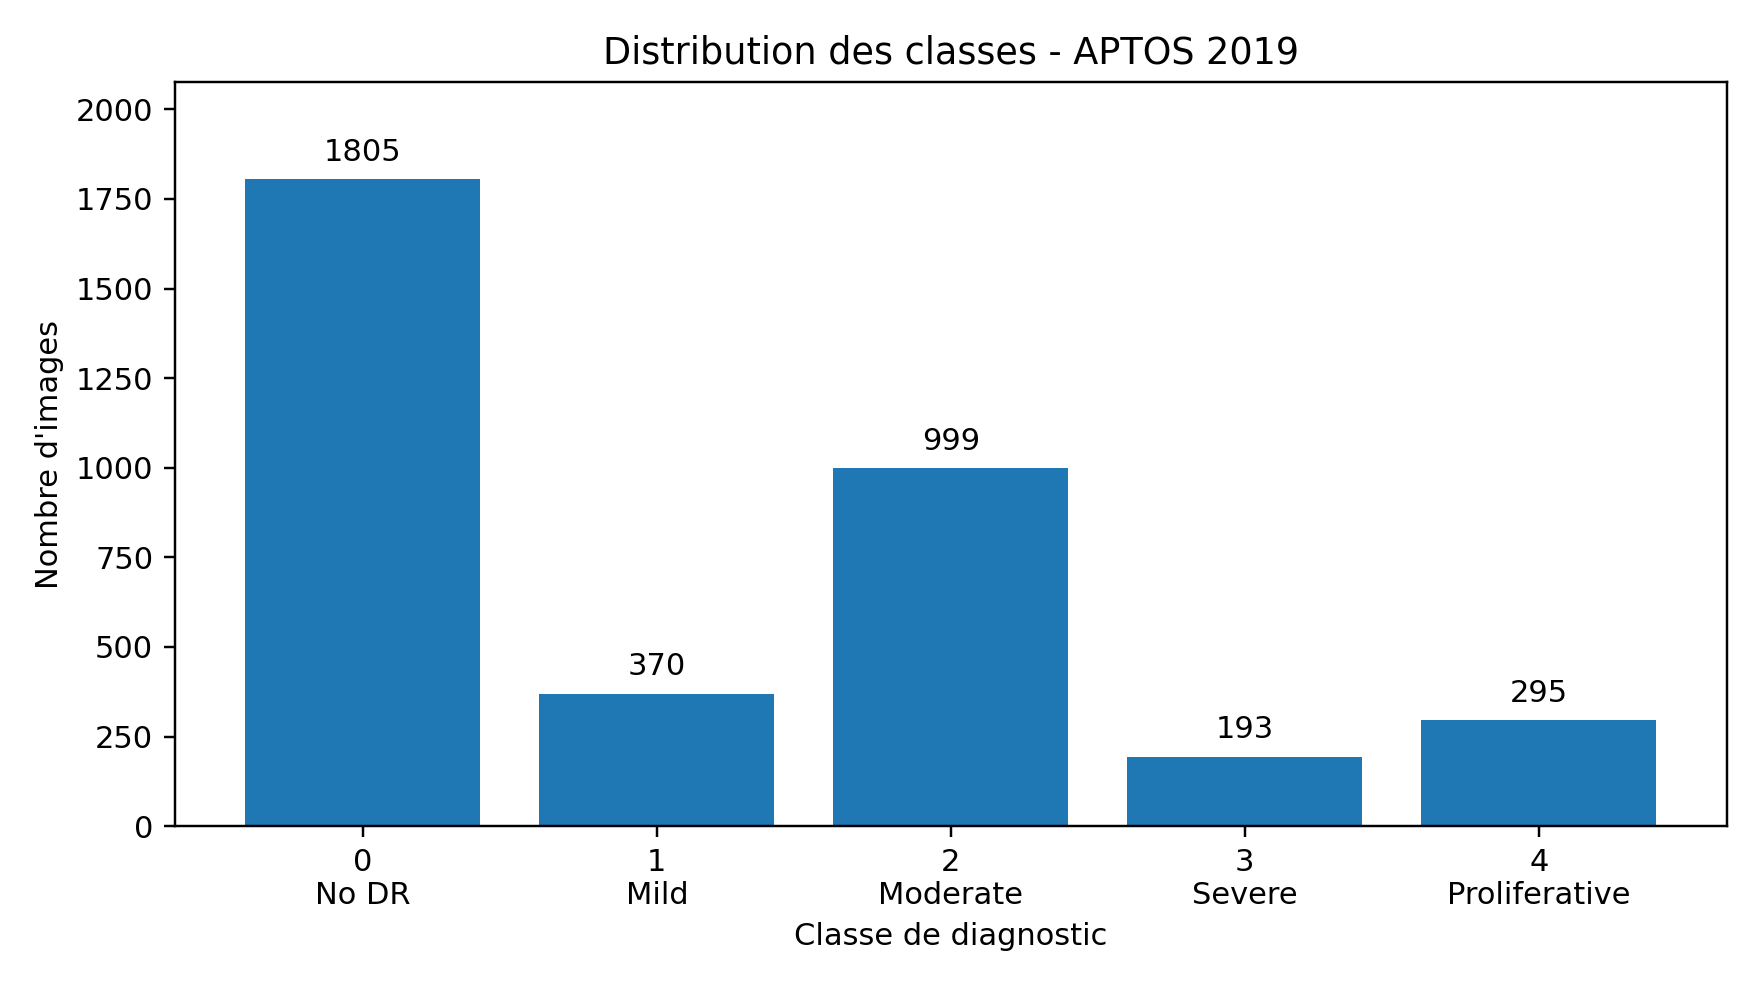
\includegraphics[width=0.88\textwidth]{class_distribution.png}
    \caption{Distribution des classes du jeu de données APTOS 2019}
    \label{fig:class_distribution}
\end{figure}

On remarque un déséquilibre important : la classe 0 est largement majoritaire, tandis que les classes 3 et 4 contiennent beaucoup moins d'images. Ce déséquilibre peut pousser le modèle à favoriser les classes fréquentes, d'où l'utilisation de techniques comme la pondération des classes et l'augmentation des données.

\section{Découpage train/validation}
Le jeu de données a été divisé en deux parties :
\begin{itemize}
    \item \textbf{80\%} pour l'entraînement, soit 2929 images ;
    \item \textbf{20\%} pour la validation, soit 733 images.
\end{itemize}

Un découpage stratifié a été utilisé afin de conserver une distribution similaire des classes dans les deux ensembles.

% =========================
\chapter{Méthodologie proposée}

\section{Pipeline général}
La figure \ref{fig:pipeline} résume le pipeline global du projet, depuis le chargement du jeu de données jusqu'à l'interface utilisateur finale.

\begin{figure}[H]
    \centering
    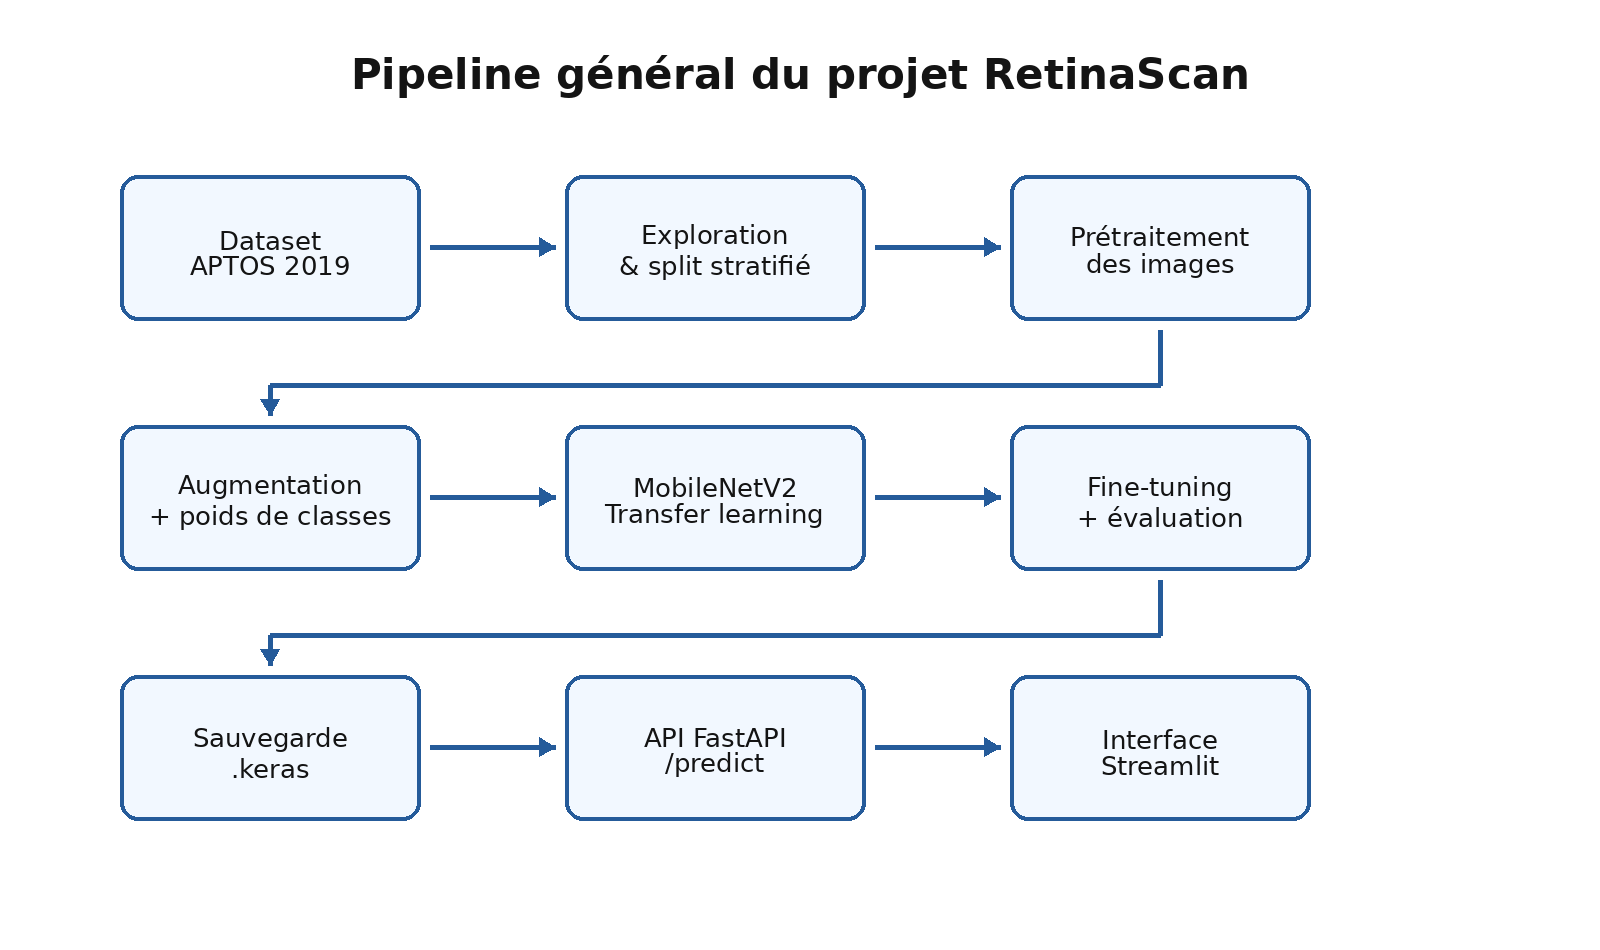
\includegraphics[width=\textwidth]{pipeline.png}
    \caption{Pipeline général du projet RetinaScan}
    \label{fig:pipeline}
\end{figure}

Le pipeline final suit la chaîne suivante : jeu de données APTOS 2019, prétraitement des images, augmentation des données, pondération des classes, extraction de caractéristiques avec EfficientNetB3, classification par une tête dense, fine-tuning, évaluation, puis déploiement avec FastAPI et Streamlit. EfficientNetB3 a été choisi comme modèle final car il offre de meilleures représentations visuelles que MobileNetV2 pour la classification d'images, tout en restant plus efficace que des architectures très lourdes.

\section{Prétraitement des images}
Les images sont chargées, converties en RGB, puis prétraitées avant d'être envoyées au modèle. Dans la version finale, les bordures noires inutiles autour du champ rétinien sont supprimées lorsque cela est possible, puis les images sont redimensionnées à une taille de \textbf{300 x 300 pixels}. Cette taille correspond à l'entrée utilisée par EfficientNetB3 dans l'implémentation finale. Les valeurs des pixels sont conservées au format \texttt{float32}, avec une plage adaptée au prétraitement interne d'EfficientNet.

\section{Augmentation des données}
Afin de réduire l'overfitting et d'améliorer la généralisation du modèle, plusieurs transformations aléatoires sont appliquées pendant l'entraînement :
\begin{itemize}
    \item retournement horizontal ;
    \item rotation légère ;
    \item zoom aléatoire ;
    \item translation légère ;
    \item variation de contraste et de luminosité lorsque la couche Keras correspondante est disponible.
\end{itemize}
Ces transformations restent modérées afin de conserver la cohérence médicale des images.

\section{Gestion du déséquilibre des classes}
Le jeu de données étant déséquilibré, des poids de classes ont été calculés avec la méthode \texttt{compute\_class\_weight}. Pour éviter des poids trop agressifs, une racine carrée des poids a été appliquée. Les poids réduits utilisés sont :

\begin{table}[H]
\centering
\caption{Pondération réduite des classes}
\label{tab:class_weights}
\begin{tabular}{cc}
\toprule
Classe & Poids utilisé \\
\midrule
0 & 0.637 \\
1 & 1.407 \\
2 & 0.856 \\
3 & 1.950 \\
4 & 1.576 \\
\bottomrule
\end{tabular}
\end{table}

\section{Architecture du modèle}
La figure \ref{fig:architecture} présente l'architecture du modèle utilisé. Le modèle final est basé sur \textbf{EfficientNetB3} en transfert learning. Le backbone EfficientNetB3 extrait les caractéristiques visuelles, puis une tête de classification dense transforme ces caractéristiques en probabilités pour les cinq classes de rétinopathie diabétique.

\begin{figure}[H]
    \centering
    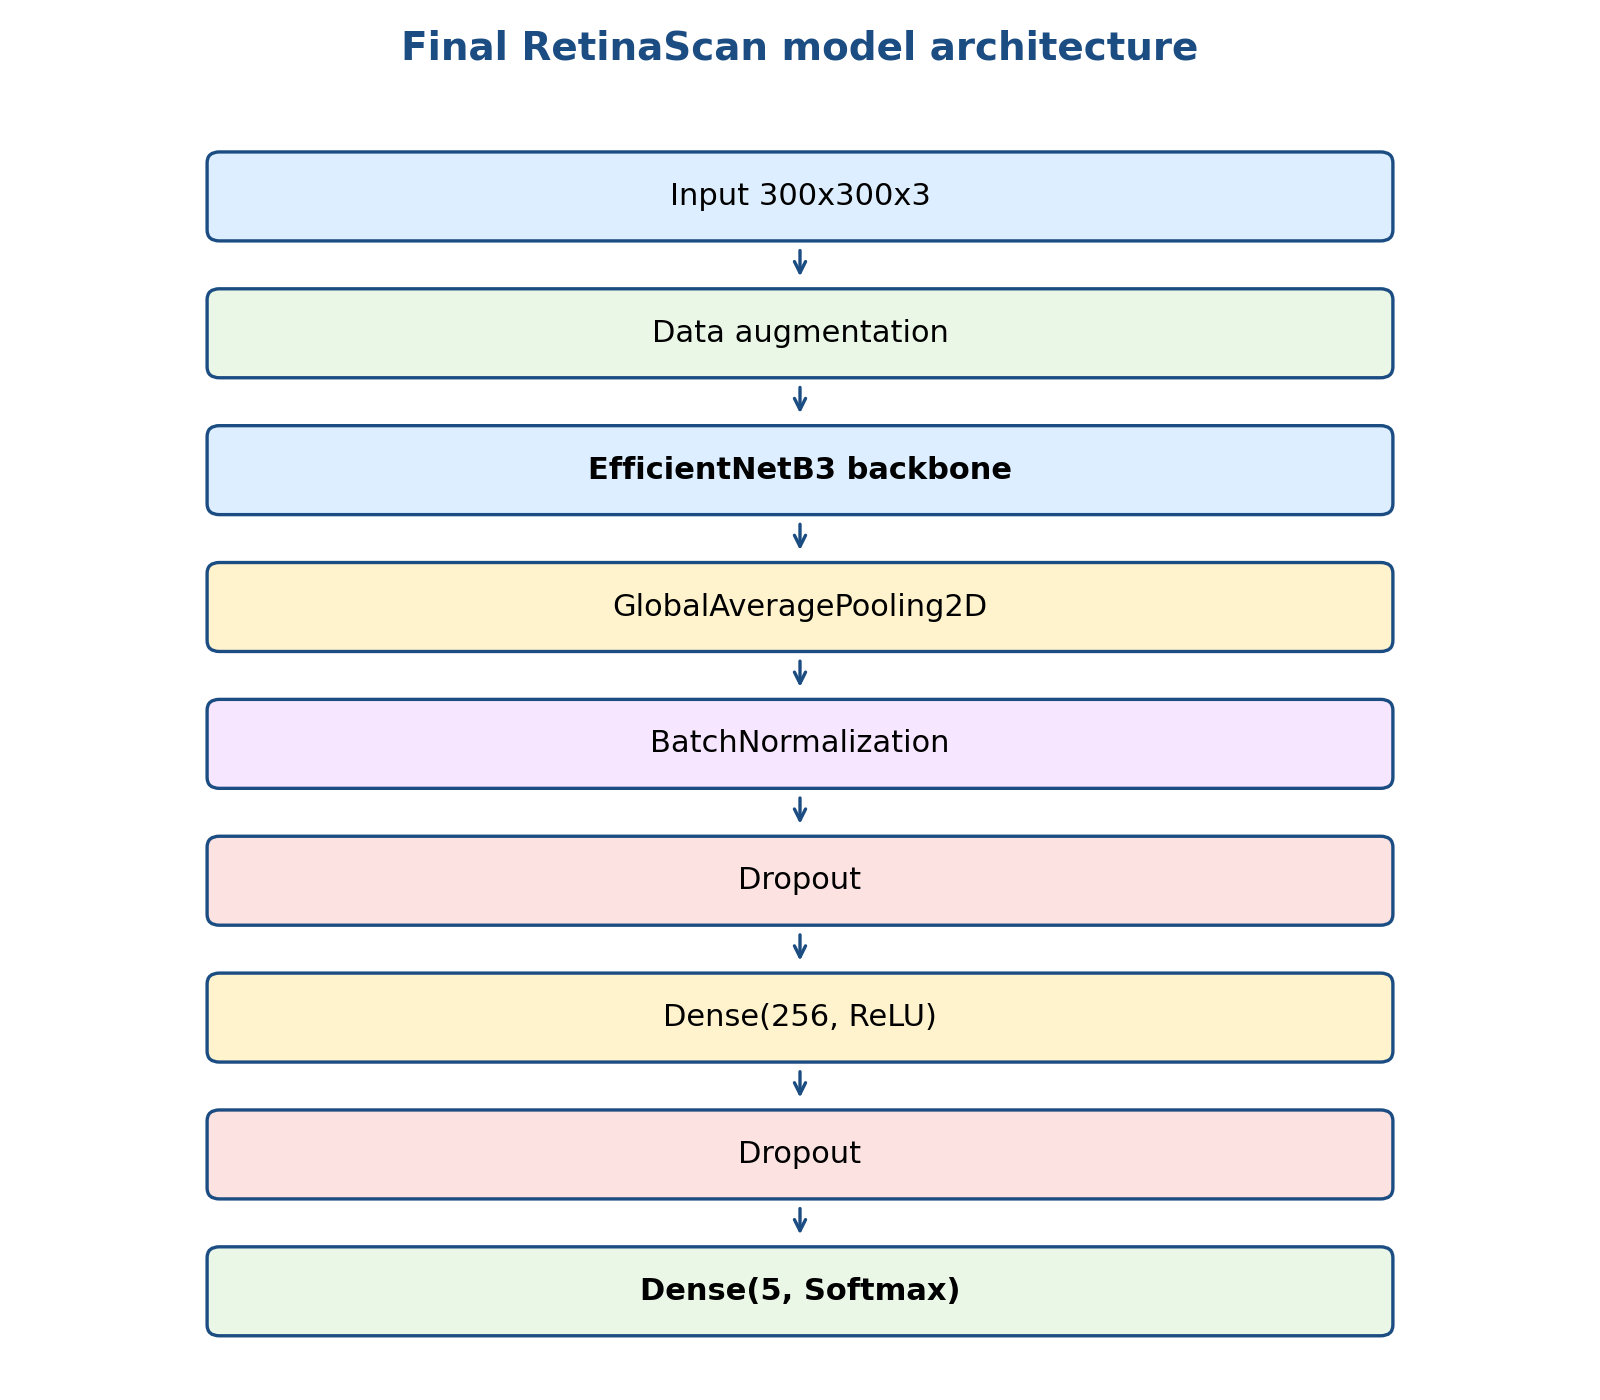
\includegraphics[width=0.98\textwidth]{model_architecture.png}
    \caption{Architecture du modèle de classification}
    \label{fig:architecture}
\end{figure}

\begin{table}[H]
\centering
\caption{Architecture du modèle final EfficientNetB3}
\label{tab:efficientnet_architecture}
\begin{tabularx}{\textwidth}{lX}
\toprule
Couche & Rôle \\
\midrule
Input \(300 \times 300 \times 3\) & Image RGB du fond d'œil prétraitée \\
Data augmentation & Flip horizontal, rotation, zoom, translation, contraste et luminosité \\
EfficientNetB3 & Backbone pré-entraîné sur ImageNet, utilisé comme extracteur de caractéristiques \\
GlobalAveragePooling2D & Conversion des cartes de caractéristiques en vecteur compact \\
BatchNormalization & Stabilisation des activations de la tête de classification \\
Dropout & Réduction du surapprentissage \\
Dense(256, ReLU) & Couche dense intermédiaire pour adapter les caractéristiques au problème \\
Dropout & Régularisation supplémentaire \\
Dense(5, Softmax) & Sortie finale correspondant aux cinq classes de rétinopathie diabétique \\
\bottomrule
\end{tabularx}
\end{table}

\section{Stratégie d'entraînement}
L'entraînement s'est déroulé en deux phases :
\begin{enumerate}
    \item \textbf{Entraînement de la tête de classification} : la base EfficientNetB3 est gelée et seules les couches ajoutées sont entraînées ;
    \item \textbf{Fine-tuning} : les dernières couches d'EfficientNetB3 sont dégélées afin d'adapter le modèle aux images de rétine.
\end{enumerate}

Les callbacks utilisés sont :
\begin{itemize}
    \item \textbf{EarlyStopping} pour éviter un surapprentissage inutile ;
    \item \textbf{ReduceLROnPlateau} pour réduire le learning rate lorsque la validation n'évolue plus ;
    \item \textbf{Best checkpoint saving} pour sauvegarder le meilleur modèle selon le Quadratic Weighted Kappa.
\end{itemize}

\section{Paramètres d'entraînement}
Le tableau \ref{tab:training_params} résume les principaux paramètres utilisés dans l'implémentation finale. Ces choix ont été faits pour garder un compromis entre performance, temps d'entraînement et simplicité de déploiement.

\begin{table}[H]
\centering
\caption{Principaux paramètres d'entraînement}
\label{tab:training_params}
\begin{tabularx}{\textwidth}{lX}
\toprule
Paramètre & Valeur utilisée \\
\midrule
Taille des images & 300 x 300 pixels \\
Batch size & 16 \\
Backbone & EfficientNetB3 pré-entraîné sur ImageNet, sans couche de classification finale \\
Tête de classification & GlobalAveragePooling2D, BatchNormalization, Dropout 0.35, Dense 256 ReLU, Dropout 0.30, Softmax 5 classes \\
Fonction de perte & \texttt{sparse\_categorical\_crossentropy} \\
Optimiseur & AdamW si disponible, sinon Adam \\
Learning rate phase 1 & 0.001 \\
Époques phase 1 & 12 au maximum, avec arrêt anticipé \\
Fine-tuning & Déblocage des dernières couches d'EfficientNetB3, avec BatchNormalization gelée \\
Learning rate fine-tuning & 0.00002 \\
Époques fine-tuning & 25 au maximum, avec arrêt anticipé \\
Réduction du learning rate & Facteur 0.3, patience 3, minimum \(10^{-7}\) \\
Meilleur checkpoint & \texttt{best\_improved\_model.keras} \\
Modèle final exporté & \texttt{retinascan\_efficientnetb3\_improved.keras} \\
\bottomrule
\end{tabularx}
\end{table}

Pendant les expériences, le déséquilibre des classes a été l'un des points les plus importants à gérer. L'utilisation directe de poids élevés peut rendre l'entraînement instable ; c'est pourquoi une version réduite des poids, basée sur la racine carrée des poids équilibrés, a été utilisée dans le rapport final.

% =========================
\chapter{Implémentation technique}

\section{Environnement de développement}
Le projet a été développé avec les outils suivants :

\begin{table}[H]
\centering
\caption{Technologies utilisées}
\label{tab:tech}
\begin{tabular}{ll}
\toprule
Technologie & Rôle \\
\midrule
Python & Langage principal \\
TensorFlow/Keras & Entraînement et sauvegarde du modèle \\
EfficientNetB3 & Backbone de classification final \\
Pandas / NumPy & Manipulation des données \\
Scikit-learn & Découpage, pondération et métriques \\
Pillow & Chargement des images \\
Matplotlib & Visualisation des résultats \\
FastAPI & API d'inférence \\
Streamlit & Interface utilisateur \\
VS Code / Conda & Environnement de développement \\
\bottomrule
\end{tabular}
\end{table}

\section{Structure du projet}
La structure finale du projet est la suivante :

\begin{lstlisting}[language=bash]
RetinaScan/
|-- aptos2019-blindness-detection/
|   |-- train.csv
|   |-- test.csv
|   |-- train_images/
|   |-- test_images/
|   |-- train_split.csv
|   |-- val_split.csv
|
|-- train_baseline.py
|-- predict_single.py
|-- api.py
|-- app.py
|-- inference_utils.py
|-- best_improved_model.keras
|-- retinascan_efficientnetb3_improved.keras
|-- train_improved.py
|-- README.md
\end{lstlisting}

Le dépôt GitHub associé au projet est disponible ici : \href{https://github.com/bilal-erraki/RetinaScan}{dépôt GitHub RetinaScan}. Il permet de partager le code avec l'encadrant et de conserver une version organisée du projet.

\section{Chargement et préparation des images}
Le pipeline de chargement des images est basé sur \texttt{tf.data}. Les images sont lues, décodées, redimensionnées puis envoyées au modèle sous forme de batches. Cette approche permet d'optimiser l'entraînement et d'éviter de charger toutes les images en mémoire.

\begin{lstlisting}[language=Python, caption={Fonction de chargement d'une image}]
def load_image(image_path, label):
    image = tf.io.read_file(image_path)
    image = tf.image.decode_png(image, channels=3)
    image = crop_black_borders(image)
    image = tf.image.resize(image, (IMG_SIZE, IMG_SIZE))
    image = tf.cast(image, tf.float32)
    return image, label
\end{lstlisting}

\section{Sauvegarde du modèle}
Le meilleur modèle EfficientNetB3 fine-tuné est sauvegardé au format natif Keras :

\begin{lstlisting}[language=Python]
model.save("best_improved_model.keras")
model.save("retinascan_efficientnetb3_improved.keras")
\end{lstlisting}

Ce format est utilisé ensuite par le script de prédiction, l'API FastAPI et l'application Streamlit.

% =========================
\chapter{Résultats expérimentaux}

\section{Métriques d'évaluation}
L'évaluation ne se limite pas à l'exactitude globale, car le jeu de données est déséquilibré. Les métriques \textbf{precision}, \textbf{recall} et \textbf{F1-score} sont donc utilisées pour analyser le comportement du modèle classe par classe. La moyenne \textit{macro} donne le même poids à chaque classe, tandis que la moyenne pondérée tient compte du nombre d'images par classe.

\section{Courbes d'entraînement}
Les figures \ref{fig:training_accuracy} et \ref{fig:training_loss} présentent l'évolution de l'exactitude et de la fonction de perte durant l'entraînement. La séparation verticale indique le passage de la phase d'entraînement de la tête de classification à la phase de fine-tuning.

\begin{figure}[H]
    \centering
    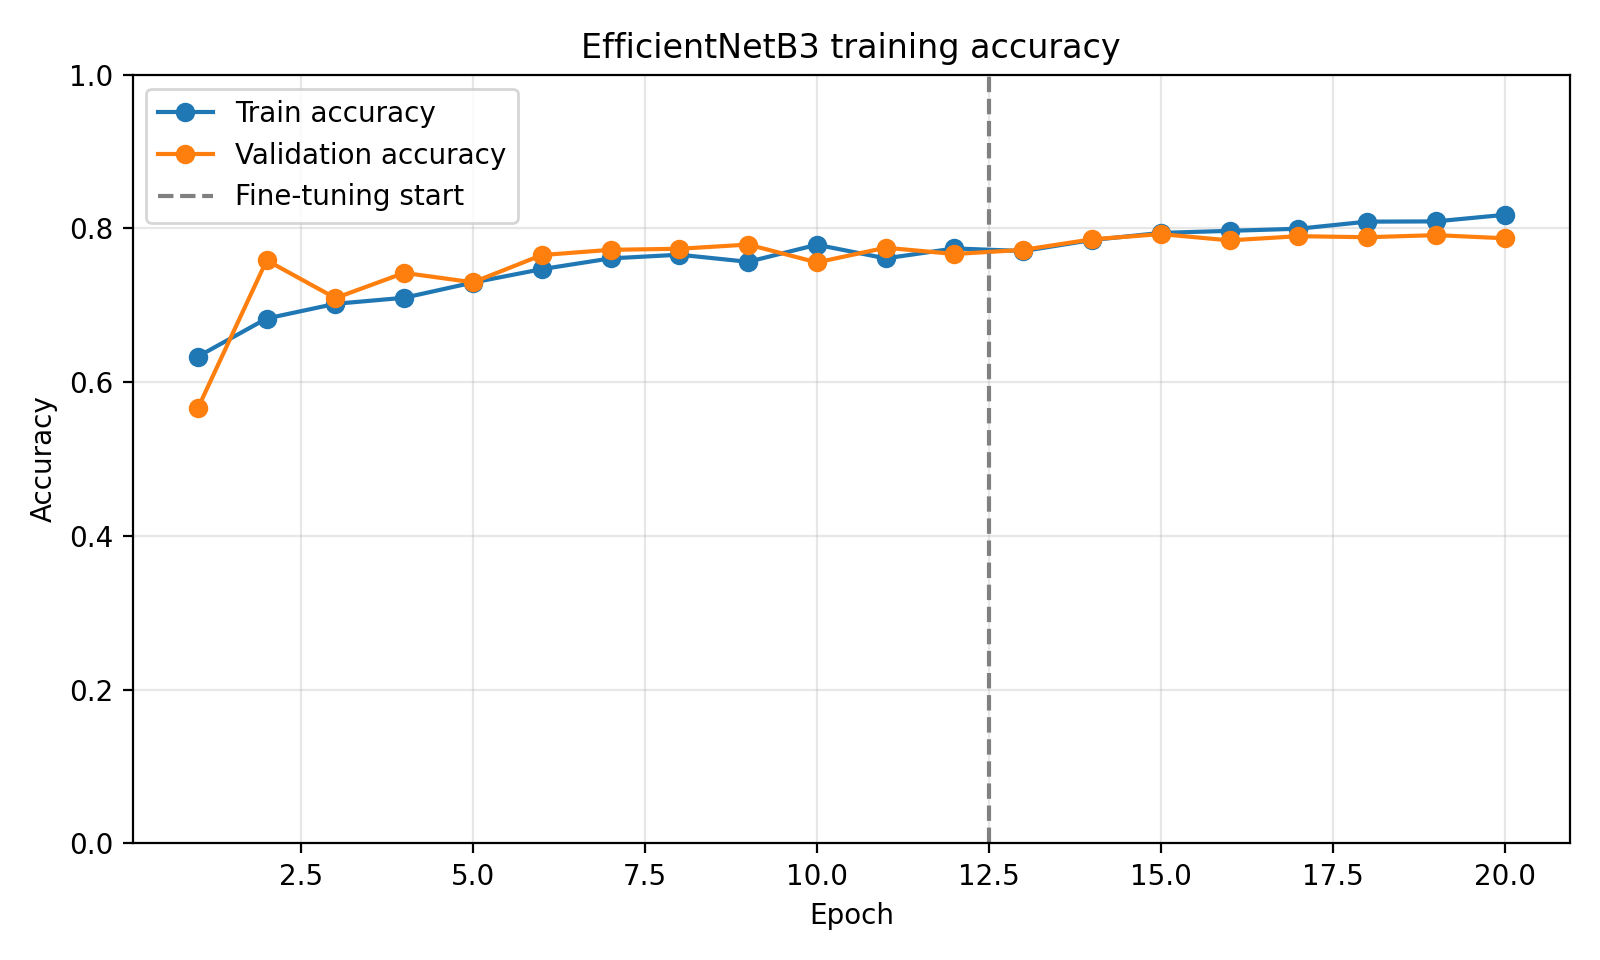
\includegraphics[width=0.9\textwidth]{training_accuracy.png}
    \caption{Évolution de l'exactitude durant l'entraînement}
    \label{fig:training_accuracy}
\end{figure}

\begin{figure}[H]
    \centering
    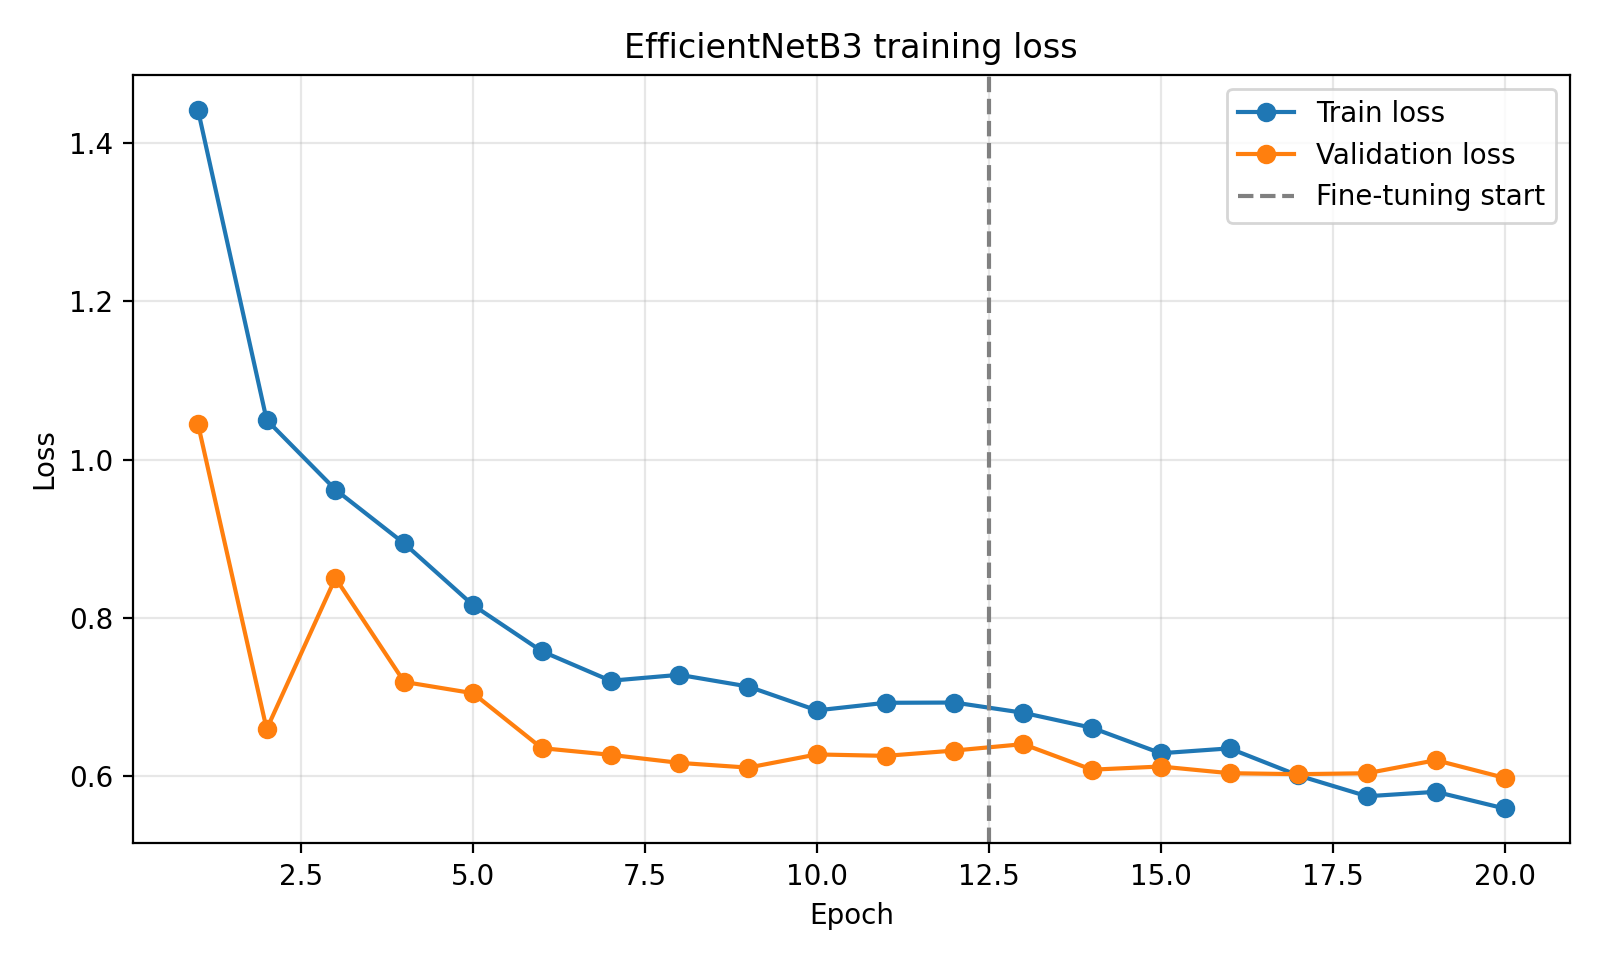
\includegraphics[width=0.9\textwidth]{training_loss.png}
    \caption{Évolution de la fonction de perte durant l'entraînement}
    \label{fig:training_loss}
\end{figure}

Le meilleur modèle EfficientNetB3 atteint une exactitude de validation de \textbf{78,58\%}, avec une perte de validation de \textbf{0,6081}. Le \textbf{Quadratic Weighted Kappa} obtenu est de \textbf{0,8603}. Cette métrique est importante dans ce projet car les stades de rétinopathie diabétique sont ordonnés : une confusion entre deux classes voisines est moins grave qu'une confusion entre une classe saine et une classe très avancée. La moyenne macro du F1-score est de \textbf{0,6021}, tandis que la moyenne pondérée du F1-score est de \textbf{0,7773}.

\section{Rapport de classification}
Le tableau \ref{tab:classification_report} présente les métriques obtenues sur l'ensemble de validation.

\begin{table}[H]
\centering
\caption{Rapport de classification sur l'ensemble de validation}
\label{tab:classification_report}
\small
\begin{tabular}{lcccc}
\toprule
Classe & Precision & Recall & F1-score & Support \\
\midrule
No DR & 0.9638 & 0.9584 & 0.9611 & 361 \\
Mild & 0.4655 & 0.3649 & 0.4091 & 74 \\
Moderate & 0.6735 & 0.8250 & 0.7416 & 200 \\
Severe & 0.4186 & 0.4615 & 0.4390 & 39 \\
Proliferative DR & 0.7143 & 0.3390 & 0.4598 & 59 \\
\midrule
Accuracy & \multicolumn{3}{c}{0.7858} & 733 \\
Macro avg & 0.6471 & 0.5898 & 0.6021 & 733 \\
Weighted avg & 0.7852 & 0.7858 & 0.7773 & 733 \\
\bottomrule
\end{tabular}
\end{table}

La performance globale est meilleure que celle de la baseline MobileNetV2. La classe \textbf{No DR} est très bien reconnue, avec un F1-score de 0,9611. La classe \textbf{Moderate} obtient également un bon rappel, égal à 0,8250. En revanche, les classes \textbf{Severe} et \textbf{Proliferative DR} restent plus difficiles, principalement à cause du déséquilibre du dataset et de la similarité visuelle entre les stades avancés.

\section{Matrice de confusion}
La matrice de confusion est présentée dans la figure \ref{fig:confusion_matrix}.

\begin{figure}[H]
    \centering
    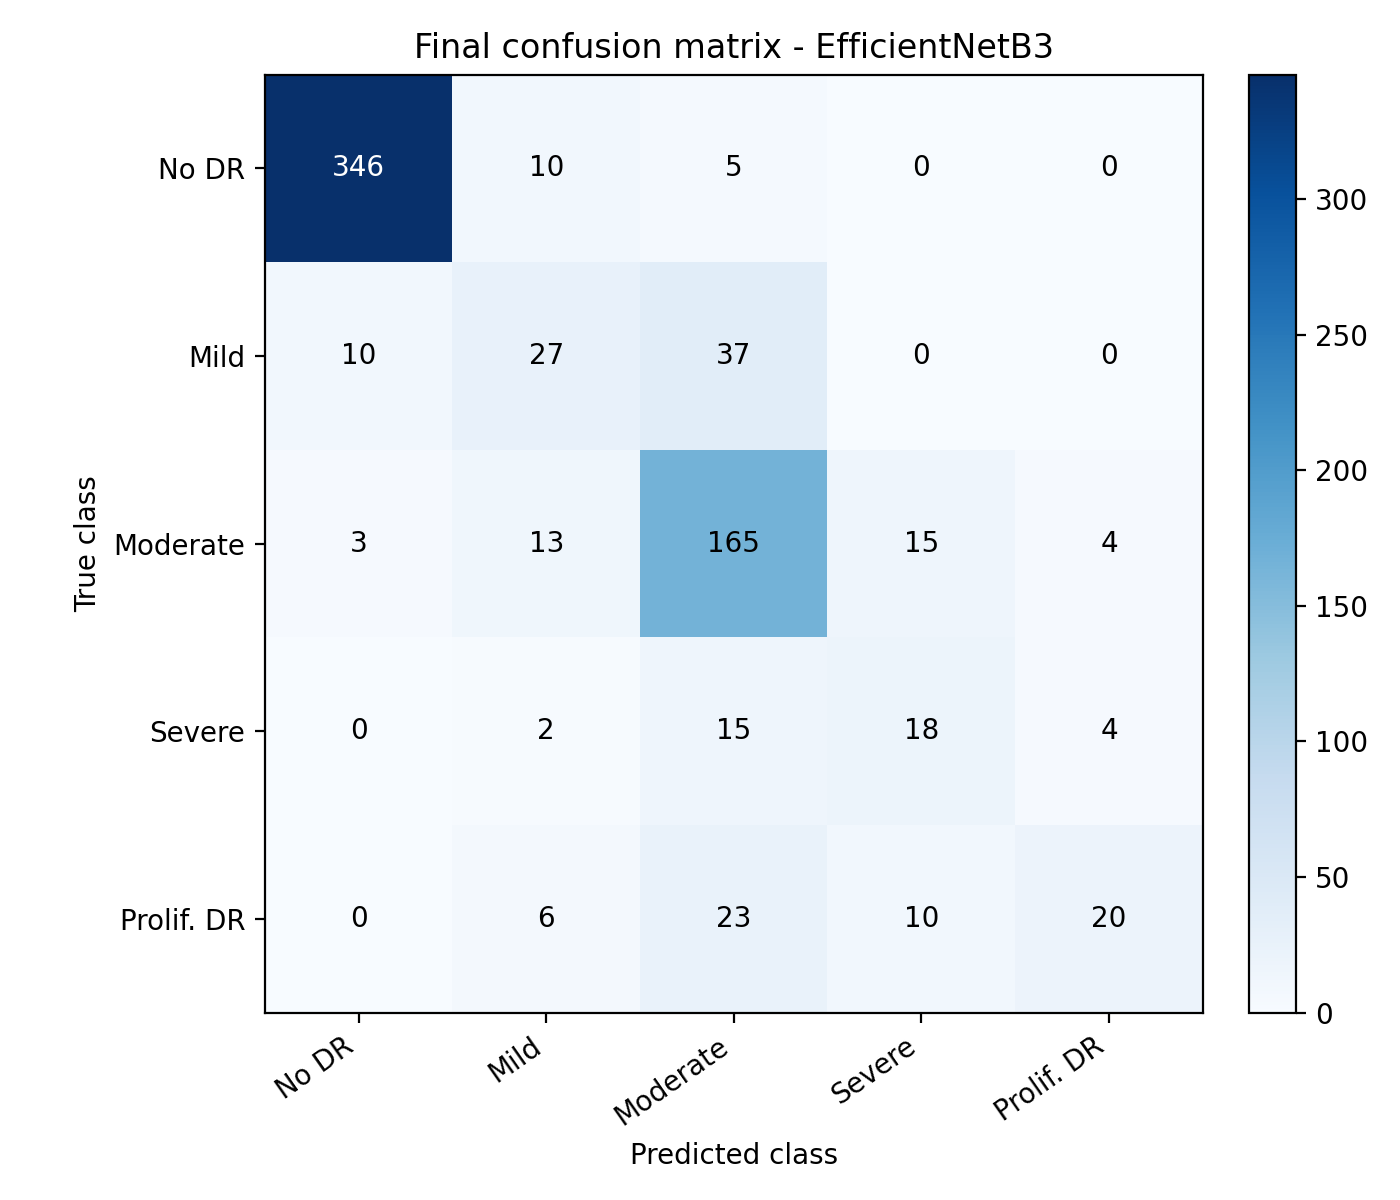
\includegraphics[width=0.78\textwidth]{confusion_matrix.png}
    \caption{Matrice de confusion du meilleur modèle}
    \label{fig:confusion_matrix}
\end{figure}

\begin{table}[H]
\centering
\caption{Matrice de confusion finale sur l'ensemble de validation}
\label{tab:confusion_matrix_values}
\small
\resizebox{\textwidth}{!}{%
\begin{tabular}{lccccc}
\toprule
Vrai / Prédit & No DR & Mild & Moderate & Severe & Prolif. DR \\
\midrule
No DR & 346 & 10 & 5 & 0 & 0 \\
Mild & 10 & 27 & 37 & 0 & 0 \\
Moderate & 3 & 13 & 165 & 15 & 4 \\
Severe & 0 & 2 & 15 & 18 & 4 \\
Prolif. DR & 0 & 6 & 23 & 10 & 20 \\
\bottomrule
\end{tabular}%
}
\end{table}

Les résultats montrent que le modèle reconnaît très bien la classe \textbf{No DR}. La classe \textbf{Moderate} est également correctement identifiée dans de nombreux cas. En revanche, les classes \textbf{Severe} et \textbf{Proliferative DR} restent plus difficiles, principalement à cause de leur faible représentation dans le jeu de données et de leur proximité visuelle avec la classe \textbf{Moderate}.

\section{Interprétation des résultats}
Le modèle donne de bons résultats pour distinguer les cas sans rétinopathie et une partie importante des cas modérés. En revanche, il ne doit pas être considéré comme fiable pour les classes sévères dans sa version actuelle. Les erreurs les plus importantes concernent les classes \textit{Severe} et \textit{Proliferative DR}, qui disposent de moins d'exemples et présentent des signes visuels parfois proches de la classe \textit{Moderate}.

Ces résultats confirment que RetinaScan doit être considéré comme un outil d'aide à la décision et non comme un outil de diagnostic médical autonome. Dans une version plus avancée, il serait utile d'ajouter un seuil de confiance et une explication visuelle des zones importantes de l'image, par exemple avec Grad-CAM.

\section{Comparaison avec la baseline}
Une première baseline basée sur MobileNetV2 avait obtenu une exactitude de validation d'environ \textbf{75,58\%}. Le modèle final EfficientNetB3 améliore cette performance avec une exactitude de validation de \textbf{78,58\%} et un Quadratic Weighted Kappa de \textbf{0,8603}. Cette amélioration montre l'intérêt d'un backbone plus puissant pour extraire des caractéristiques visuelles plus discriminantes.

\begin{table}[H]
\centering
\caption{Comparaison entre la baseline et le modèle final}
\label{tab:baseline_comparison}
\begin{tabular}{lcc}
\toprule
Modèle & Validation accuracy & Quadratic Weighted Kappa \\
\midrule
MobileNetV2 baseline & 75,58\% & -- \\
EfficientNetB3 final & 78,58\% & 0,8603 \\
\bottomrule
\end{tabular}
\end{table}

L'amélioration globale reste modérée en exactitude, mais elle est importante pour l'évaluation ordinale du problème. EfficientNetB3 améliore la performance globale et apporte de meilleurs résultats sur certains stades avancés, même si les classes Severe et Proliferative DR restent les plus difficiles.

% =========================
\chapter{Déploiement de la solution}

\section{Script de prédiction}
Un script de prédiction simple, \texttt{predict\_single.py}, a d'abord été développé pour tester le modèle sur une image. Ce script charge le modèle sauvegardé, prépare l'image à la taille attendue par le réseau, effectue une prédiction et affiche la classe prédite ainsi que les probabilités associées. Dans la version finale, le backend charge en priorité \texttt{best\_improved\_model.keras}. Le modèle exporté complet est également disponible sous le nom \texttt{retinascan\_efficientnetb3\_improved.keras}.

\section{API FastAPI}
L'API FastAPI permet d'exposer le modèle EfficientNetB3 à travers un endpoint \texttt{/predict}. L'utilisateur envoie une image, l'API la convertit en RGB, applique le prétraitement rétinien, la redimensionne en \textbf{300 x 300}, exécute le modèle, puis retourne une réponse JSON contenant :
\begin{itemize}
    \item la classe prédite ;
    \item le label textuel ;
    \item le niveau de confiance ;
    \item les probabilités de chaque classe.
\end{itemize}

\begin{lstlisting}[language=Python, caption={Extrait simplifié du endpoint de prédiction}]
@app.post("/predict")
async def predict(file: UploadFile = File(...)):
    image = preprocess_image(await file.read(), image_size=300)
    probabilities = model.predict(image)[0]
    predicted_class = int(np.argmax(probabilities))

    return {
        "predicted_class": predicted_class,
        "predicted_label": class_names[predicted_class],
        "confidence": round(float(np.max(probabilities)) * 100, 2),
        "probabilities": {
            class_names[i]: float(probabilities[i])
            for i in range(len(class_names))
        }
    }
\end{lstlisting}

La documentation interactive générée par FastAPI permet de vérifier rapidement les routes disponibles et le format exact de la réponse. La figure \ref{fig:swagger_overview} montre la page Swagger avec la route d'accueil et le endpoint de prédiction. La figure \ref{fig:swagger_response} illustre un test réel du endpoint \texttt{/predict} avec une image envoyée en \texttt{multipart/form-data} et une réponse JSON contenant les probabilités de chaque classe.

\textit{Remarque : les captures d'écran Swagger et Streamlit servent à illustrer le fonctionnement du déploiement. Elles peuvent provenir de sessions de test différentes et ne doivent pas nécessairement être comparées comme le résultat d'une même image.}

\begin{figure}[H]
    \centering
    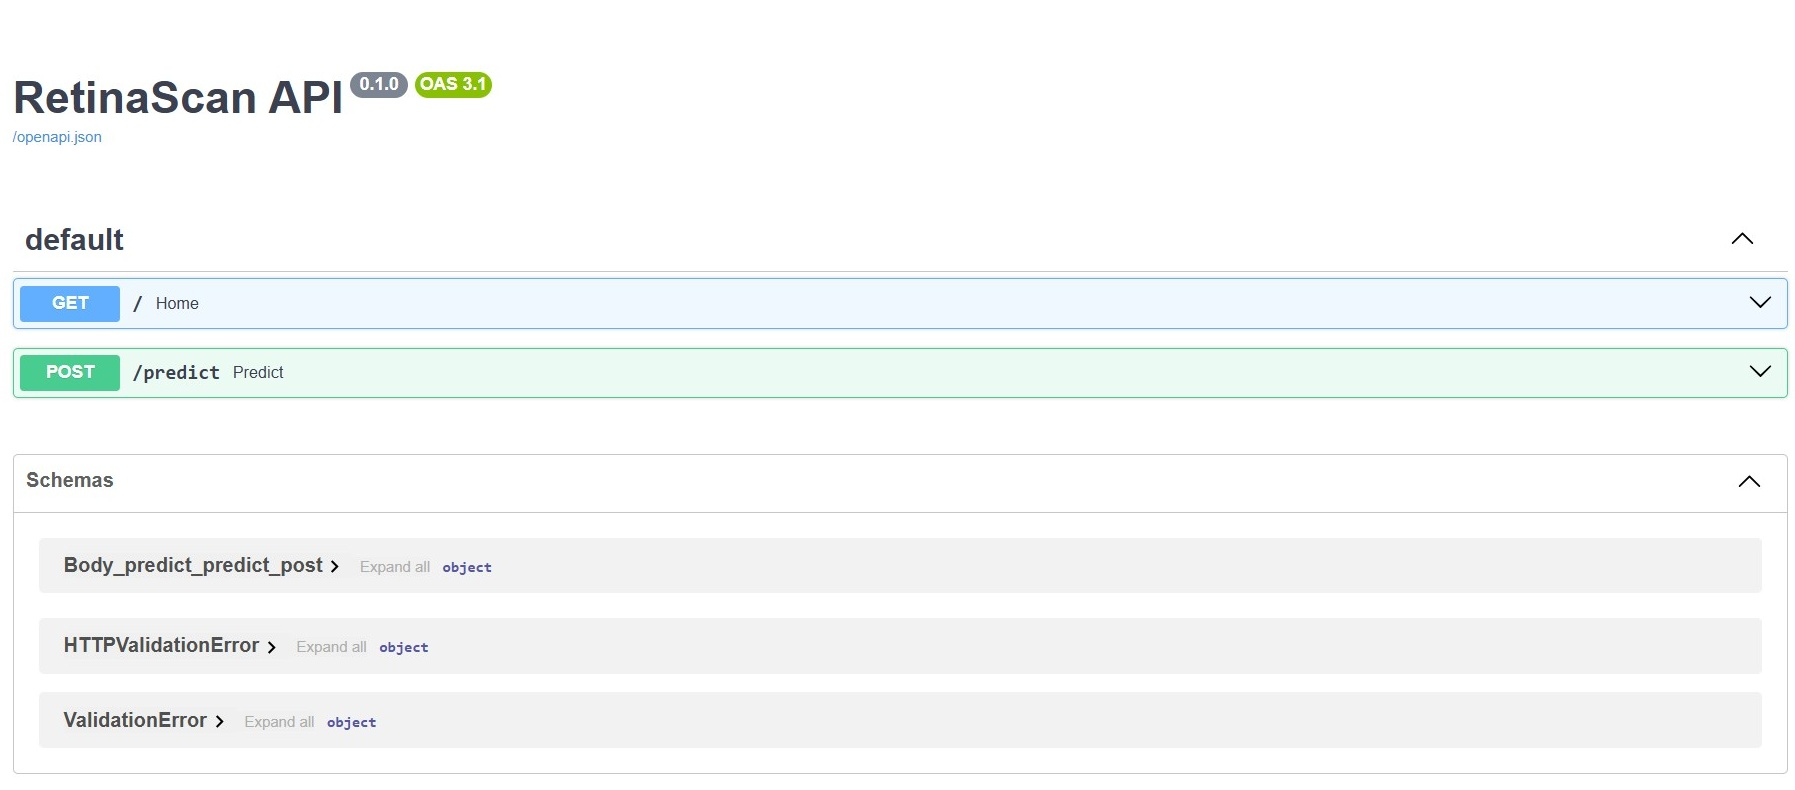
\includegraphics[width=0.98\textwidth]{swagger_overview.jpg}
    \caption{Documentation Swagger de l'API RetinaScan}
    \label{fig:swagger_overview}
\end{figure}

\begin{figure}[H]
    \centering
    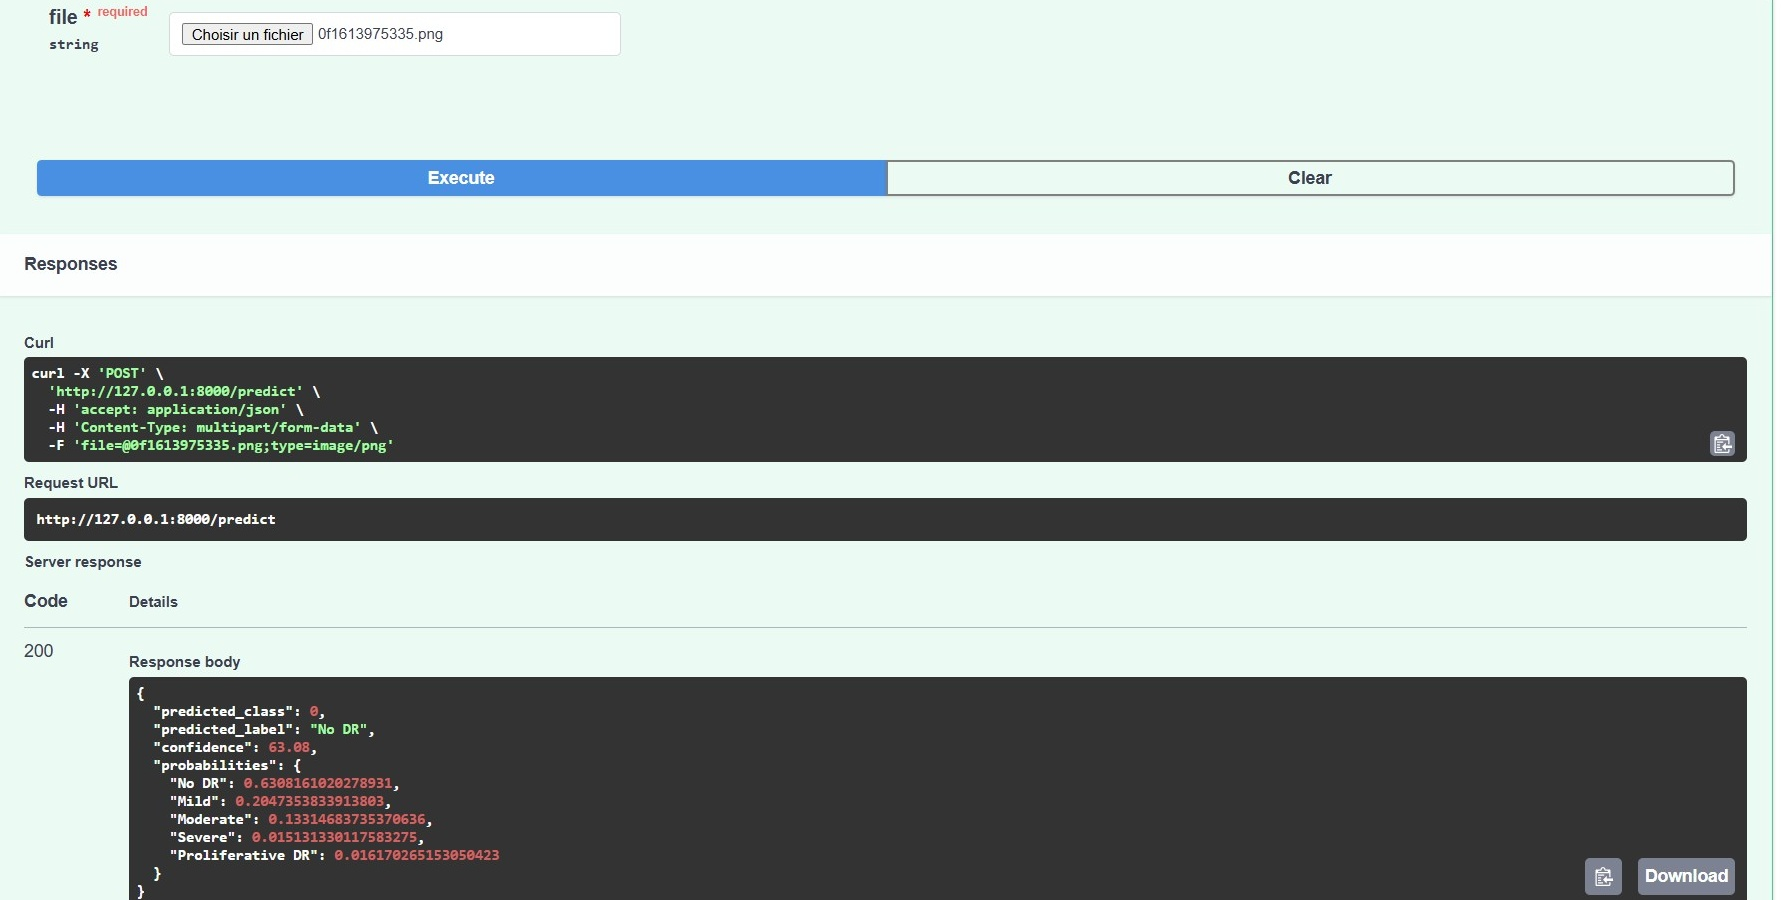
\includegraphics[width=0.98\textwidth]{swagger_predict_response.jpg}
    \caption{Test du endpoint de prédiction dans Swagger UI}
    \label{fig:swagger_response}
\end{figure}

\section{Interface Streamlit}
L'interface Streamlit permet à l'utilisateur de téléverser une image du fond d'œil, d'appeler l'API et d'afficher le résultat sous forme claire. Les probabilités de chaque classe sont affichées avec des barres de progression, ce qui rend la sortie du modèle plus compréhensible pour l'utilisateur. Un message d'avertissement rappelle que le résultat fourni par le modèle ne remplace pas un diagnostic médical.

\begin{figure}[H]
    \centering
    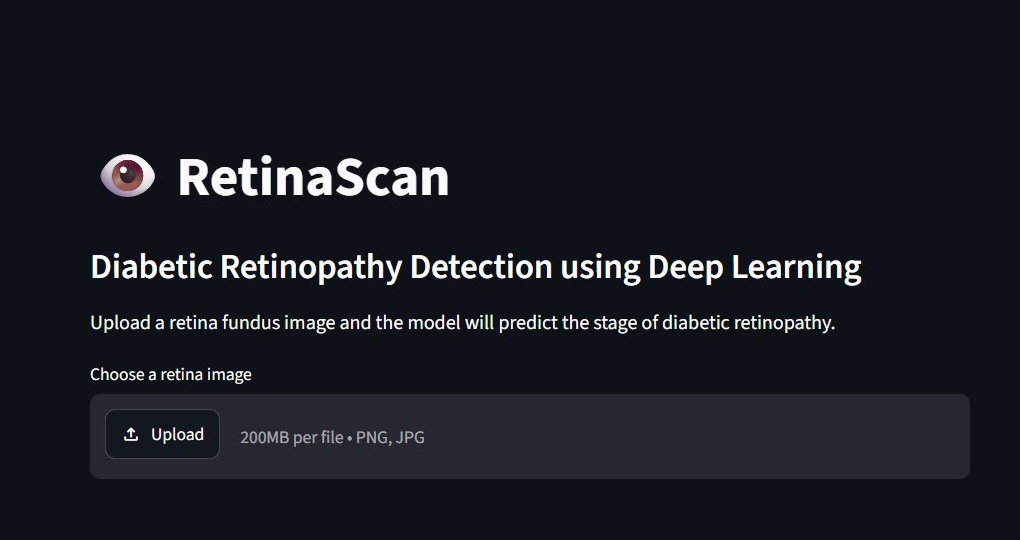
\includegraphics[width=0.98\textwidth]{streamlit_home.jpg}
    \caption{Page d'accueil de l'application Streamlit}
    \label{fig:streamlit_home}
\end{figure}

\begin{figure}[H]
    \centering
    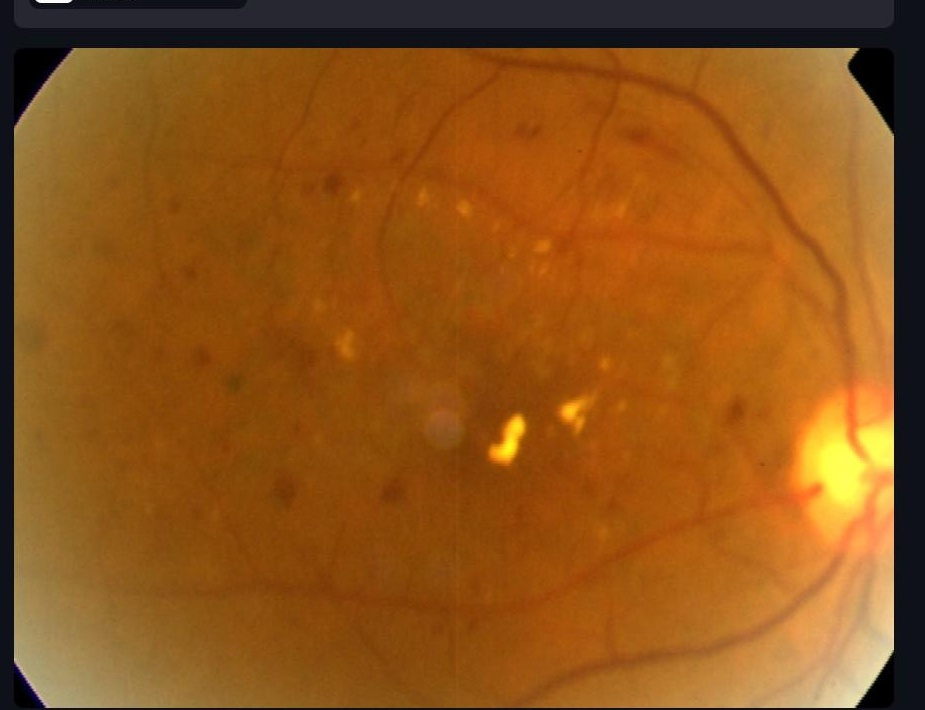
\includegraphics[width=0.98\textwidth]{streamlit_uploaded_image.jpg}
    \caption{Prévisualisation de l'image rétinienne téléversée}
    \label{fig:streamlit_uploaded_image}
\end{figure}

\begin{figure}[H]
    \centering
    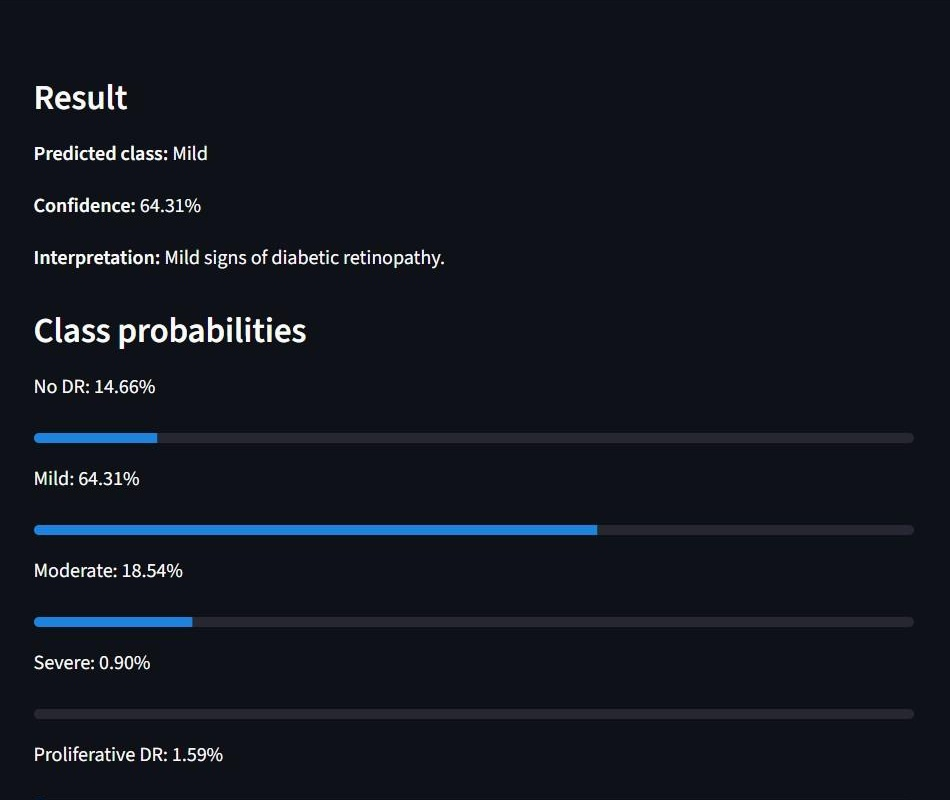
\includegraphics[width=0.98\textwidth]{streamlit_prediction_result.jpg}
    \caption{Affichage de la classe prédite et des probabilités dans Streamlit}
    \label{fig:streamlit_prediction_result}
\end{figure}

\section{Commandes d'exécution}
Le code source complet est organisé dans le \href{https://github.com/bilal-erraki/RetinaScan}{dépôt GitHub RetinaScan}.

L'API est exécutée avec la commande suivante :

\begin{lstlisting}[language=bash]
python -m uvicorn api:app --reload
\end{lstlisting}

L'interface Streamlit est exécutée dans un deuxième terminal :

\begin{lstlisting}[language=bash]
python -m streamlit run app.py
\end{lstlisting}

% =========================
\chapter{Limites et perspectives}

\section{Limites du projet}
Même si le système fonctionne correctement, plusieurs limites doivent être signalées :
\begin{itemize}
    \item le jeu de données est déséquilibré, ce qui réduit la performance sur les classes rares ;
    \item les classes sévères sont parfois confondues avec la classe Moderate ;
    \item l'entraînement a été réalisé sur CPU, ce qui limite le nombre d'expériences possibles ;
    \item le modèle n'a pas été validé cliniquement ;
    \item l'application est une démonstration académique et non un dispositif médical.
\end{itemize}

\section{Améliorations possibles}
Plusieurs pistes peuvent être envisagées pour améliorer le projet :
\begin{itemize}
    \item ajouter une explicabilité visuelle avec Grad-CAM afin d'indiquer les zones de l'image qui influencent la prédiction ;
    \item entraîner et évaluer le modèle sur des jeux de données plus larges et plus variés ;
    \item améliorer la gestion des classes Severe et Proliferative DR avec de l'oversampling, des pertes adaptées ou davantage de données ;
    \item entraîner le modèle sur GPU afin d'augmenter le nombre d'expériences ;
    \item ajouter une gestion explicite de l'incertitude dans l'interface ;
    \item déployer l'application sur un serveur ou une plateforme cloud.
\end{itemize}

% =========================
\chapter{Conclusion}
Le projet \textbf{RetinaScan} a permis de développer une solution complète de classification de la rétinopathie diabétique à partir d'images du fond d'œil. Le travail réalisé couvre toutes les étapes d'un projet de Deep Learning appliqué : exploration du jeu de données, préparation des données, entraînement du modèle, évaluation, sauvegarde, API d'inférence et interface utilisateur.

Le modèle final basé sur EfficientNetB3 et le fine-tuning a obtenu une exactitude de validation de \textbf{78,58\%} et un Quadratic Weighted Kappa de \textbf{0,8603}. Ces résultats améliorent la baseline MobileNetV2 et confirment l'intérêt d'un backbone plus puissant pour la classification d'images rétiniennes. L'analyse détaillée montre cependant que les classes rares restent le principal point faible du système.

Le travail réalisé m'a permis de comprendre qu'un bon score global ne suffit pas dans un problème médical : il faut analyser les erreurs classe par classe, utiliser des métriques adaptées comme le Quadratic Weighted Kappa, expliquer les limites et éviter de présenter le modèle comme un outil de diagnostic autonome. Le système final est fonctionnel de bout en bout : entraînement, sauvegarde du modèle, API FastAPI et interface Streamlit. Les perspectives principales concernent l'ajout de Grad-CAM, l'utilisation de jeux de données plus larges, une meilleure prise en charge des classes Severe et Proliferative DR, ainsi qu'un déploiement cloud.

% =========================
\appendix
\chapter{Annexe : résumé des résultats}

\begin{table}[H]
\centering
\caption{Résumé des principaux résultats}
\begin{tabular}{lc}
\toprule
Élément & Valeur \\
\midrule
Nombre d'images d'entraînement & 3662 \\
Taille train split & 2929 \\
Taille validation split & 733 \\
Nombre de classes & 5 \\
Backbone & EfficientNetB3 \\
Meilleur modèle & best\_improved\_model.keras \\
Modèle final exporté & retinascan\_efficientnetb3\_improved.keras \\
Validation accuracy & 78,58\% \\
Validation loss & 0,6081 \\
Quadratic Weighted Kappa & 0,8603 \\
Macro F1-score & 0,6021 \\
Weighted F1-score & 0,7773 \\
Dépôt GitHub & \href{https://github.com/bilal-erraki/RetinaScan}{RetinaScan} \\
\bottomrule
\end{tabular}
\end{table}

\chapter{Annexe : avertissement médical}
RetinaScan est un projet académique destiné à démontrer l'utilisation du Deep Learning pour l'analyse d'images médicales. Les prédictions fournies par le modèle ne constituent pas un diagnostic médical. Toute interprétation réelle doit être réalisée par un professionnel de santé qualifié.

% =========================
\begin{thebibliography}{9}

\bibitem{aptos}
APTOS 2019 Blindness Detection, Kaggle Competition. Dataset d'images du fond d'œil pour la détection de la rétinopathie diabétique.
\url{https://www.kaggle.com/competitions/aptos2019-blindness-detection}

\bibitem{gulshan2016}
Gulshan, V. et al. Development and Validation of a Deep Learning Algorithm for Detection of Diabetic Retinopathy in Retinal Fundus Photographs. JAMA, 2016.

\bibitem{he2016}
He, K., Zhang, X., Ren, S., Sun, J. Deep Residual Learning for Image Recognition. IEEE/CVF Conference on Computer Vision and Pattern Recognition, 2016.

\bibitem{huang2017}
Huang, G., Liu, Z., Van Der Maaten, L., Weinberger, K. Q. Densely Connected Convolutional Networks. IEEE/CVF Conference on Computer Vision and Pattern Recognition, 2017.

\bibitem{tan2019}
Tan, M., Le, Q. EfficientNet: Rethinking Model Scaling for Convolutional Neural Networks. International Conference on Machine Learning, 2019.

\bibitem{mobilenetv2}
Sandler, M., Howard, A., Zhu, M., Zhmoginov, A., Chen, L.-C. MobileNetV2: Inverted Residuals and Linear Bottlenecks. IEEE/CVF Conference on Computer Vision and Pattern Recognition, 2018.

\bibitem{tensorflow}
TensorFlow Documentation. Framework open-source pour le Machine Learning et le Deep Learning.
\url{https://www.tensorflow.org/}

\bibitem{fastapi}
FastAPI Documentation. Framework Python pour la création d'API modernes.
\url{https://fastapi.tiangolo.com/}

\bibitem{streamlit}
Streamlit Documentation. Framework Python pour construire des interfaces web interactives.
\url{https://streamlit.io/}

\bibitem{githubrepo}
ERRAKI Bilal. RetinaScan GitHub Repository.
\url{https://github.com/bilal-erraki/RetinaScan}

\end{thebibliography}

\end{document}
